%!TEX root = ../../Master.tex
\section{Algorithms for pathfinding}

Constructing a model of the real world in math can be done by graph, finding the shortest path from one vertex to another, can be defined as single-pair shortest path problem. Finding the shortest path from vertex $u$ to vertex $v$. Algorithms for solving such problem, which are able to search through a graph for a solution. Searching a graph means systematically following edges in a graph thereby visiting vertices in a graph. Graph search algorithms differentiate themselves by their method of searching through a graph. Algorithms like dijkstra's algorithm are for solving single-source shortest path problem, finding a the shortest path from a source, to all other vertices in a graph. Backtracking from a specific vertex back to the source, it is possible to find the shortest path from a start vertex A to a destination vertex B in a graph \cite{Cormen2009}. Graph search algorithms are more effective than others in finding the shortest path connecting two vertices in a graph. This section describes both Dijkstra's algorithm in \cref{subs_dijkstra} and the A* algorithm in \cref{subs_astar}. These algorithms are very much alike, but they each have different assets. For example; Dijkstra's algorithm always finds the shortest path. However it is it inefficient in terms of speed in finding the shortest path. The A* algorithm will always find the shortest path, just like Dijkstra, given the heuristic value that is supplied is admissible. This is discussed in \cref{subs_astar}. A* differs from Dijkstra in terms of how fast the shortest path is evaluated.

%   In \cref{sec:specification} we specified that our solution needs to find the shortest weighted path to the destination.
%   To better understanding pathfinding we examined different algorithms. We discovered that some algorithms have a high accuracy but is slow at finding the path, and conversely.
%   We have compared some well known path finding algorithms by evaluating their calculation time and route precision.

%   In the following we compare 3 frequently used algorithms:
%   \begin{itemize}
%     \setlength{\itemsep}{1pt}
%     \setlength{\parskip}{0pt}
%     \setlength{\parsep}{0pt}
%     \item \textbf{Dijkstra's Algorithm} Always finds the shortest path but has long calculation time on more complex graphs.
%     \item \textbf{Greedy Best-First-Searches} Is a very fast algorithm but does not always find the shortest path.
%     \item \textbf{A* Algorithm} Is an extension of Dijkstra's Algorithm but has less calculation time using heuristic values.
% \end{itemize}

% The A* algorithm was chosen as the algoritm of choice because it always finds the shortest path, and still has a reasonable fast computing time. This algorithm also makes it easier to implement stairs and elevators, because of the heuristic values. In this section we will describe A* and Dijkstra's because A* is an extension of Dijkstra's.


  %Path finding algorithms are used for finding a path between two locations, the source and the destination. By searching its way from the source to the destination, until a path is found. These algorithms also make it possible to calculate the optimal path, i.e. the shortest. \cite{Cormen2009}


  \begin{figure}[ht!]
    \centering
    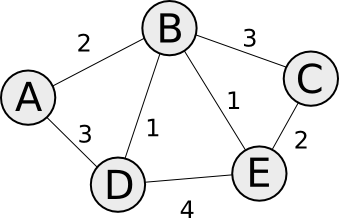
\includegraphics[width=0.5\textwidth]{Graph}
    \caption{Weighted graph}
    \label{fig:graph}
  \end{figure}

  %An important factor of a searching algorithm is correctness and also the time required to calculate the optimized path. The algorithms can be rated by their worst-case time, to ensure a responsive performance.

  \subsection{Dijkstra's Algorithm}\label{subs_dijkstra}


  A commonly used algorithm for finding the shortest path is Dijkstra's algorithm. It loops through steps until all vertices to the target vertex is optimized with the least cost, then points out the shortest path from source vertex, to target vertex. Because of the need of every vertex being evaluated, see \cref{fig:dijkstra}, the complexity of algorithm is proportional to the number of vertices, which means that a lot of computational power is required to calculate the result. \cite{Dijkstr1959}

  \begin{figure}[ht!]
    \centering
    \frame{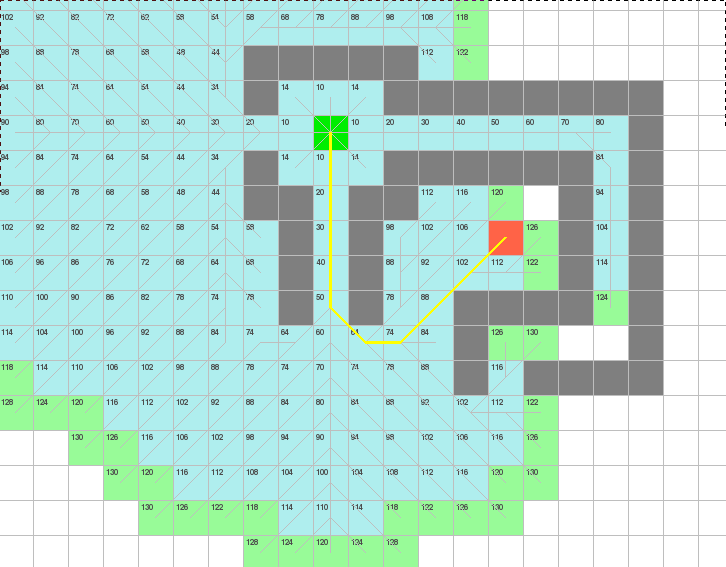
\includegraphics[width=0.5\textwidth]{Dijkstra}}
    \caption{Dijkstra's algorithm in action}
    \label{fig:dijkstra}
  \end{figure}

\begin{algorithm} \label{algo:Dij}
  \caption{Dijkstra's Algorithm}
  \KwResult{Finds the shortest path from start vertex to Vertices}
  \KwData{\\
  graph \tcc*{graph containing vertices}
  source \tcc*{the source vertex to start evaluating from}
  dist \tcc*{list of distances from source}
  visited \tcc*{list of visited vertices}
  previous \tcc*{list of vertices with shortest parent}
  Q \tcc*{A list vertices to be evaluated}
  v \tcc*{evaluating vertex}
  u \tcc*{current vertex}
  }

  \SetKwFunction{Dijkstra}{Dijkstra}
  \SetKwProg{KwFn}{Function}{}{}

  \KwFn{\Dijkstra{graph, source}}{

    \For{\textbf{each} vertex v in graph}{
      dist[$v$] $\gets \infty$\tcc*{Assign distance from source to as infinite}
      visited[$v$] $\gets$ false\tcc*{Boolean to false for not visited}
      previous[$v$] $\gets$ undefined\tcc*{Assign previous all as undefined}
    }

    dist[$source$] $\gets 0$\tcc*{Source dist has distance 0}
    insert $source$ in $Q$\tcc*{Source dist has distance 0}

    \While{Q \textbf{is not} empty}{
      $u \gets$ vertex $v$ in $Q$ with lowest dist[]\tcc*{The new $u$ is the vertex with lowest dist value}
      remove $u$ from $Q$\tcc*{Remove vertex $u$ from $Q$}
      visited[$u$] $\gets$ true\tcc*{Mark the new vertex $u$ as visited}

      \For{\textbf{each} neighbour v of u}{
        $alt \gets$ dist[$u$] + distBetween($v$, $u$)\tcc*{Assign the cost to $v$ from $source$ added the weight between $v$ and $u$}
        \If{alt < dist[v]\tcc*{If $alt$ is lower than the already assign dist value for vertex $v$}}{
          dist[$v$] $\gets alt$\tcc*{Store the shortest distance to vertex $v$ from $source$}
          previous[$v$] $\gets u$\tcc*{Store the short parent $u$ to current vertex $v$}
          \If{!visited[v]}{
            insert $v$ into $Q$\tcc*{Add the unvisited $v$ into the $Q$ to be evaluated}
          }
        }
      }
    }
    return dist\tcc*{Return the distances in dist}
  }
\end{algorithm}

\begin{algorithm} \label{algo:FindPath}
  \caption{Find path to target}
  \KwResult{Finds the shortest path from start vertex to a target vertex}
  \KwData{\\
        stack \tcc*{Empty sequence}
        target \tcc*{Target vertices}
        source \tcc*{Source vertex}
        u \tcc*{evaluating vertices}
        previous \tcc*{A list of parents with lowest cost from source}
   }

  \SetKwFunction{FindPath}{FindPath}
  \SetKwProg{KwFn}{Function}{}{}

  \KwFn{\FindPath{previous, source, target}}{
    $u \gets target$\;
    $stack \gets$ empty sequence\;
    \While{previous[u] \textbf{is not} source}{
      insert $u$ in stack\tcc*{Insert u vertex in the stack}
      $u \gets$ previous[$u$]\tcc*{Traverse from target to source}
    }
    return
  }
\end{algorithm}

  % We consider the problem: find shortest path from source to target.

  % Where $P$ is the source vertex, $Q$ is the target and $R$ is the evaluating vertex.

  % The vertices are subdivided into three sets:

  % \begin{description}
  %   \item[Set $A$]{Optimized vertices (least costly path from $P$ is known)}
  %   \item[Set $B$]{Temporary vertices (evaluated cost of path from $P$ but not part of set $A$)}
  %   \item[Set $C$]{Remaining vertices}
  % \end{description}

  % The edges are subdivided into three other sets:

  % \begin{description}
  %   \item[Set \RN{1}]{Edges used in the set $A$}
  %   \item[Set \RN{2}]{Not part of set I (one and only one edge of this set will lead to each vertex in set $B$)}
  %   \item[Set \RN{3}]{Remaining edges (rejected or not yet considered)}
  % \end{description}

  % At first all vertices is assigned to set $C$ and all edges to set \RN{3}, P is then assigned to set $A$.
  % Then we loop through following steps until $Q$ is part of set $A$. R is the evaluating vertex, and r is the connected edge.

  % \begin{description}
  %   \item[Step 1.]{Consider all the edges r connecting the vertex just assigned to set $A$. If $R$ is part of set $C$ assign to set $B$ and assign edge r to set \RN{2}. If vertex R is part of set $B$, then investigate if the use of edge r is less costly from $P$ to R than the existing edge in set \RN{2}. If less costly assign edge r and reject existing edge in set \RN{2}, otherwise reject r to set \RN{3}.}
  %   \item[Step 2.]{For each vertex in set $B$ where there is only one path in set \RN{1} and set \RN{2}, the vertex with minimum cost from $P$ is assign to set $A$ and with the corresponding edge assign to set \RN{1}.}
  % \end{description}



  % In this example \cref{fig:dijkstra_calc}, the first vertex B is assigned to set $A$, and edge $AB$ is part of set \RN{1}.

  % \begin{figure}[ht!]
  %   \centering
  %   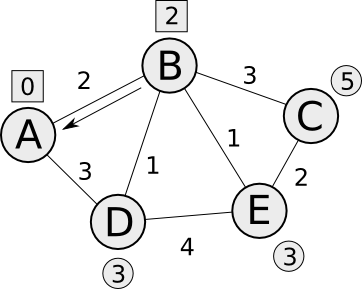
\includegraphics[width=0.5\textwidth]{DijkstraX}
  %   \caption{Dijkstra calculation}
  %   \label{fig:dijkstra_calc}
  % \end{figure}

  \subsection{A* Algorithm}\label{subs_astar}


  The A* algorithm is an extension to Dijkstra's algorithm described in \cref{subs_dijkstra} providing better performance in terms of speed, while still maintaining the correctness of Dijkstra's algorithm.

  \subsubsection{Cost function}
  The cost function $g(x)$ is simply calculated by adding the g value of the previous vertex to the g value of the current vertex.

  \subsubsection{Heuristic function and evaluation function}
  A* introduces a heuristic value. In pathfinding the heuristic value is commonly based on the distance from the current vertex A* is checking to the goal vertex. Many different methods of finding this distance exists. Some of the typically used distance functions are the Manhattan distance and the Euclidean distance. The heuristic value is used when determining the evaluation function $f(x) = g(x) + h(x)$, where $g(x)$ describes the cost from the start to the vertex being evaluated, and $h(x)$ is the heuristic function. The evaluation function is the value used when determining if a vertex is in the shortest path. When comparing two vertices for shortest path, the vertex with the lowest f value is always chosen \cite{Patel2013}.

  When calculating the heuristic function, 4 situations can occur which affects the performance of A*.

    \begin{itemize}
    \item If $h(x)$ is zero, then only $g$ affects the result essentially making it work like Dijkstra's algorithm.

    \item If $h(x) < g(x)$, the algorithm will guaranteed find the shortest path from source to target but at a slow running time. This is because if the heuristic value is small, it does not affect the evaluation function and A* would traverse the graph in the wrong way relative to the goal.

    \item $h(x) = g(x)$, the algorithm will only extract the best path if there are no obstacles blocking the shortest path. If there are obstacles, A* will not be able to search the graph for paths around the obstacles.

    \item If $h(x) > g(x)$, the algorithm will find a path very fast but not always the shortest path, because A* will depend too much on the heuristic value to give a qualified shortest path.
  \end{itemize}

  When considering these 4 situations, $h(x)$ should be admissible, meaning that the heuristic value should never overestimate the distance between the evaluating vertex and the target vertex. In contrast it should be just right for the final chosen path to be the optimal path and for the complexity of the algorithm to be at a minimum. 

  For an example of an A* calculation, see \cref{fig:astar}. 
  Grey blocks are obstacles such as walls. White blocks are unvisited vertices. S marks the start and G the goal. Blue blocks mark vertices that were added to closed set (were visited) and green blocks mark vertices that were added to open set (were considered to be added to closed set). A marks a point where the heuristic value increases because the distance to G increases, causing the evaluation value to rise above the threshold for when A* considers another path. Point B marks a point where A* chooses a path around an obstacle.

  \paragraph{Euclidean distance}\cite{wiki_euclidean}

  \[
    dist(p, q) = dist(q, p) = \sqrt{(q_{1} - p_{1})^2 + (q_{2} - p_{2})^2 + \dots + (q_{n} - p_{n})^2}
  \]

  Where $p$ and $q$ both are vertices in a graph. $p_{n}$ and $q_{n}$ are the coordinates of each vertices. For example $p_{1}$ is the $x$ coordinate of vertex $p$.

    \paragraph{Manhattan distance}\cite{wiki_manhattan_distance}

  \[
    dist(p, q) = dist(q, p) = \| \mathbf{p} - \mathbf{q} \| = \sum\limits_{i=1}^n | \mathbf{p_{i}} - \mathbf{q_{i}} |
  \]

  Where $p$ and $q$ both are vertices in a graph. $p_{n}$ and $q_{n}$ are the coordinates of each vertices. For example $p_{1}$ is the $x$ coordinate of vertex $p$.

  % If you would combine Dijkstra's algorithm with Best-First-Search algorithm, you would get the A* algorithm which also utilises the principle of a heuristic estimation to determine which vertex to test next. It uses a evaluation function $f(x) = g(x) + h(x)$, where $g(x)$ describes the cost from the start to the vertex being evaluated, and $h(x)$ is a heuristic function that estimates the cost from the evaluating vertex to the target vertex. \cite{Patel2013}


\begin{algorithm} \label{algo:A*}
  \caption{A* Algorithm}
  \KwResult{Finds the shortest path from start vertex to goal vertex}
  \KwData{ \\
    source  \tcc*{the source vertex to start evaluating from} 
    goal \tcc*{the goal vertex to find path to} 
    closedSet = \{ \} \tcc*{set of visited vertices} 
    openSet = \{ start \} \tcc*{the set of vertices to be evaluated} 
    cameFrom = \{ \} \tcc*{list of navigated vertices} 
    gScore[] = \tcc*{array containing every g value for every vertex} 
    fScore[] = \tcc*{array containing every f value for every vertex} 
    current = \tcc*{current vertex being evaluated} 
    neighborNodes(vertex) = \tcc*{set of neighbors for every vertex}
    hEstimate(vertex1,vertex2) \tcc*{function that calculates heuristic value from vertex1 to vertex2. Could use euclidean distance}
    distBetween(vertex1,vertex2) \tcc*{gets cost from vertex1 to vertex2}
    }

  \SetKwFunction{Astar}{Astar}
  \SetKwProg{KwFn}{Function}{}{}

  \KwFn{\Astar{start, goal}}{

    gScore[start] $\gets 0$ \tcc*{Set cost from start to 0}

    fScore[start] $\gets $ gScore[start] $+$ hEstimate(start,goal) \tcc*{Set f value of start vertex}

    \While{openSet \textbf{is not} empty}{
      current $\gets$ vertex in openSet having the lowest fScore value\;
      
      \tcc{if current is goal, goal is reached}
      \If{current $=$ goal}{ 


        return reconstructPath(cameFrom, goal) \tcc*{goal is reached so reconstruct path and return it}
        }
      }
    
    \tcc{remove current vertex from openSet and add to closedSet}
    remove current from openSet \;
    add current to closedSet\;

    \For{\textbf{each} neighbor in neighborNodes(current)}{
      tempGScore $\gets$ gScore[current] + distBetween(current,neighbor)\;

      tempGScore $\gets$ tempGScore + hEstimate(neighbor,goal)\;

      \tcc{if neighbor is in closedSet and tempFScore $>=$ f value of neighbor, continue}
      \If{neighbor in closedSet and tempFScore $>=$ fScore[neighbor]}{
        continue\;
      }

      \If{neighbor not in openSet or tempFScore $<$ fScore[neighbor]}{
        cameFrom[neighbor] $\gets$ current\;
        gScore[neighbor] $\gets$ tempGScore\;
        fScore[neighbor] $\gets$ tempFScore\;
        \If{neighbor not in openSet}{
          add neighbor to openSet\;
        }
      }
    }

return failure\tcc*{if this point is reached, the goal vertex is never reached}
  }

\end{algorithm}

\begin{algorithm} \label{algo:reconstructPath}
  \caption{Reconstruct path}
  \KwResult{reconstructs the shortest path from start vertex to a target vertex}
  \KwData{\\
        stack \tcc*{Empty sequence}
        target \tcc*{Target vertices}
        source \tcc*{Source vertex}
        u \tcc*{evaluating vertices}
        previous \tcc*{A list of parents with lowest cost from source}
   }

  \SetKwFunction{ReconstructPath}{ReconstructPath}
  \SetKwProg{KwFn}{Function}{}{}

  \KwFn{\ReconstructPath{cameFrom, currentVertex}}{

    \If{currentNode in cameFrom}{
      p $\gets$ reconstructPath(cameFrom, cameFrom[currentVertex])
      return (p currentVertex)
    }
    $u \gets target$\;
    $stack \gets$ empty sequence\;
    \While{previous[u] \textbf{is not} source}{
      insert $u$ in stack\tcc*{Insert u vertex in the stack}
      $u \gets$ previous[$u$]\tcc*{Traverse from target to source}
    }
    return
  }
\end{algorithm}

\sinote{reconstruct path algorithm skal lige skrives færdig}


  \begin{figure}[ht!]
    \centering
    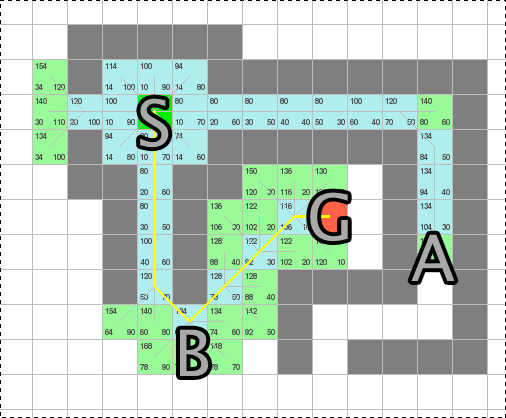
\includegraphics[width=0.5\textwidth]{AstarHlow_kopi.png}
    \caption{A* algorithm with an admissible heuristic value. }
    \label{fig:astar}
  \end{figure}

  % There are multiple ways to calculate the heuristic value(estimated cost) to the target vertex, but an ideal choice would be the Euclidean \cref{equation:Euclidean} distance, as no path can be shorter than the direct distance between two vertices.
  % \begin{equation} \label{equation:Euclidean}
  %   dist((x, y), (a, b)) = \sqrt{(x - a)^2 + (y - b)^2}
  % \end{equation}

  \subsection{Summary of Algorithms}

  Path algorithms searches for a path to target. Some focuses on finding a path fast, others finding the most optimal path. Using the A* algorithm with a heuristic model that is admissible, which underestimates the cost to the target path, assure an optimal path without calculating every vertex. See \cref{tbl:scheme}.
  
  \begin{table}[ht!]
    \centering
  \rowcolors{1}{}{lightgray}
    \begin{tabular}{|r|l|c|}

      \hline
      \textbf{Algorithm} & \textbf{Advantages} & \textbf{Disadvantages} \\
      \hline
      Dijkstra's & Always optimal path & Slow calculation \\
      Best-First-Search & Fast calculation & Not always optimal path \\
      A* & Optimal path if $h(x)<g(x)$, Fast calculation & Not always optimal path \\
      \hline
    \end{tabular}
    \caption{Table of advantages/disadvantages of different algorithms}
    \label{tbl:scheme}
  \end{table}